% Auf der Basis von dem Springer llncs Style
\documentclass{llncs}					% Springer Style
\usepackage{llncsdoc}					% Springer Dokument
\usepackage[utf8]{inputenc}				% Umlaute, Sonderzeichen
\usepackage[ngerman]{babel}				% deutsche Sprache
\usepackage{enumitem}					% Listen
\usepackage{graphicx}					% Grafiken
\usepackage{hyperref}					% Hyperlinks
\usepackage[nonumberlist]{glossaries}	% Glossar

\bibliographystyle{unsrt}

\makenoidxglossaries

%\newglossaryentry{Aktuator}{
%	name=Aktuator,
%	plural=Aktuatoren,
%	description={Bauelement, welches elektrische Signale in andere physikalische Größen, wie beispielsweise Bewegung, umsetzt.}
%}

%\newglossaryentry{TrackingAufgabe}{
%	name=Tracking Aufgabe,
%	plural=Tracking Aufgaben,
%	description={Aufgabe, bei der über einen gewissen Zeitraum ein Parameter durchgehend angepasst werden muss.\newline Bsp. Mauszeiger, der innerhalb eines sich verändernden Bereiches des Computer-Monitors gehalten werden muss.}
%}

\title{Aufmerksamkeitssteuerung durch Haptische Schnittstellen in Überwachungstätigkeiten}
\author{Leon Huck\thanks{Unter der Betreuung von: Erik Pescara}}
\institute{Karlsruher Institut für Technologie}
\date{17.06.2019}

\begin{document}
	
%Titel der Arbeit
\maketitle

%Schlagworte der Arbeit
\begin{description}
	\item 
\end{description}

%Abstrakt der Arbeit
%\begin{abstract}
	
%\end{abstract}

%Inhaltsverzeichnis
%ToDo: Überdenken, ob nicht entfernen
\newpage
\tableofcontents
\newpage

%Hinführung zu der Arbeit
\clearpage
\section{Einleitung}

Seit der Einführung von Geräten, wie etwa Handies, sind Aufmerksamkeitshinweise durch Vibrationen im Alltag angekommen. So kann das Handy auch in lauten Umgebungen auf neue Mitteilungen aufmerksam machen. Gleichzeitig werden die Mitmenschen nicht durch durchdringende Töne gestört.

Doch bieten haptische Informationen auch außerhalb von einem einfachen Alarmsystem, wie es im besagten Handy zu finden ist, eine Vielzahl an Möglichkeiten zur Informationsübermittlung (vgl. \cite{10.2307/1705360}). Diese Möglichkeiten zu untersuchen ist Ziel dieser Arbeit.

Um das Ziel zu erreichen werden Definitionen für Aufmerksamkeitssteuerung und Überwachungsaufgaben eingeführt um anschließend deren Schnittmenge zu betrachten. Dabei werden die Teilbereiche anhand von konkreten Anwendungen erarbeitet und die allgemeinen Erkenntnisse herausgezogen.
Dadurch soll der Stand der Wissenschaft festgehalten und potentielle Forschungsfragen aufgedeckt werden.

\clearpage
%Beschreibung der Teilgebiete, die im späteren Verlauf zusammengeführt werden
\section{Die Thematischen Teilgebiete}

\begin{figure}[htbp]
	\begin{center}
		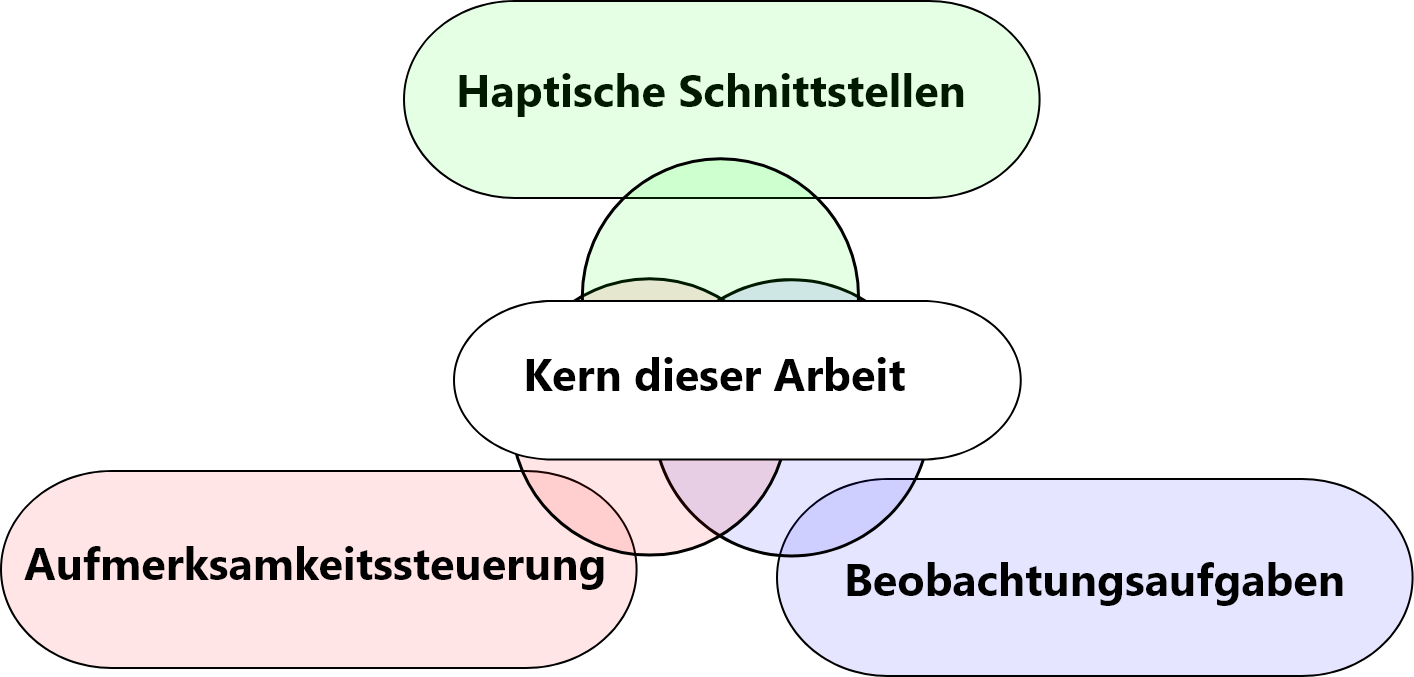
\includegraphics[width = 8cm]{Grafiken/Venn-Diagramm.png}
		\caption{Graphische Darstellung der Teilgebiete und deren Interaktion anhand eines Venn-Diagramm.}
		\label{Venn-Diagramm.png}
	\end{center}
\end{figure}

Um eine Diskussion über die möglichen Anwendungen von haptischen Schnittstellen bei der Aufmerksamkeitsbeeinflussung während Beobachtungsaufgaben zu führen ist es unerlässlich die Themenbereiche genau abzugrenzen. Der Grund hierfür ist die Mehrfachverwendung der einzelnen Begriffe. Demzufolge werden die in verwendeten Definitionen vorgestellt.

\subsection{Aufmerksamkeitssteuerung}

\begin{figure}[htbp]
	\begin{center}
		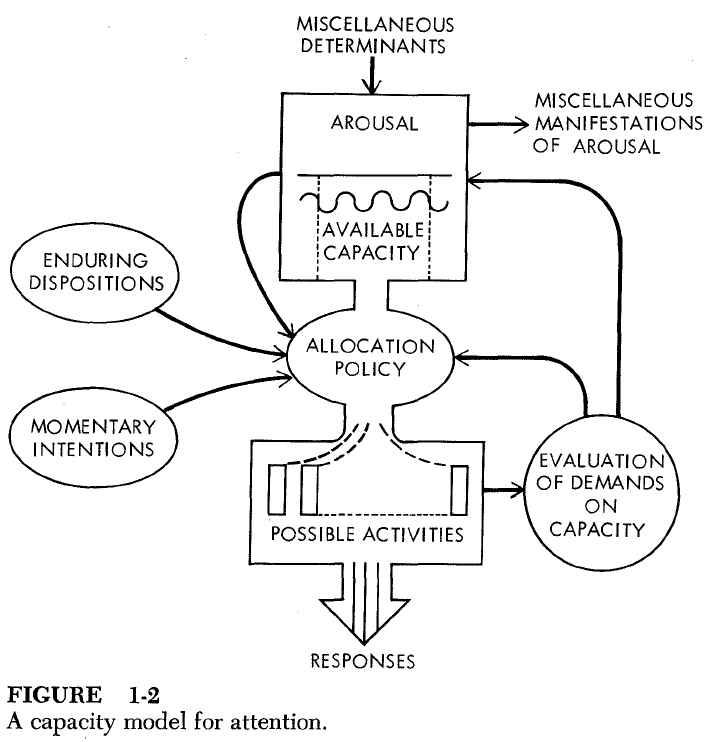
\includegraphics[width = 5cm]{Grafiken/28-Attention-Model.png}
		\caption{Das Zusammenwirken von Aufmerksamkeit und dem Erregungszustand eines Menschen zur Bildung einer Entscheidung\cite{kahneman1973attention}.}
		\label{28-Attention-Model}
	\end{center}
\end{figure}

Die menschliche Arbeitskraft ist begrenzt. Das gilt insbesondere für die kognitiven Fähigkeiten eines Menschen. Jede Aktion die ausgeführt oder durchdacht werden soll verbraucht Energie und Zeit. Bereits vermeidlich einfache Aktionen benötigen diese beiden Ressourcen. Deshalb muss es einen Mechanismus beziehungsweise ein Handlungsvorschrift geben, nach der die Ressourcen auf die unterschiedlichen Aufgaben verteilt werde. Diese Vorschrift heißt Aufmerksamkeit.
 Daniel Kahneman \cite{kahneman1973attention} beschreibt unterschiedliche Eigenschaften der Aufmerksamkeit.
 
 	\paragraph{Selektierungs-Eigenschaft der Aufmerksamkeit}
 	Alle Organismen, und somit auch Menschen, müssen unterscheiden, welche Stimulationen wichtig und welche unwichtig sind. Werden zwei Berührungen gleichzeitig wahrgenommen muss entschieden werden, welche Information Priorität hat. Geschiet dies nicht können unerwünschte Konsequenzen folgen. So muss in kürze entschieden werde, ob eine juckende Stelle nur ein unbedeutendes Haar oder ein giftiges Insekt ist. Diese Unterscheidungen benötigen ebenfalls Aufmerksamkeit.
 	
 	\paragraph{Intensitäts-Eigenschaft der Aufmerksamkeit} 	
 	Die Aufmerksamkeit ist nicht entweder vorhanden oder nicht vorhandenen. Sie bewegt sich auf einem Spektrum.
 	Kahneman\cite{kahneman1973attention} führt hierfür das Beispiel eines Schülers an, der dem Unterricht folgt. Es gibt für dem Schüler nicht die Möglichkeit seine vollständige Aufmerksamkeit auf den Unterricht zu lenken. Täte er dies hätte er keine Möglichkeiten mehr auf Änderungen in seiner Umgebung zu reagieren. Auch könnte er nicht entscheiden, wann es sinnvoll wäre, eine andere Aufgabe zu beginnen. Gleichzeitig kann er nicht dem Unterricht vollständig ignorant begegnen. Wenn er dies könnte müsste er gleichzeitig in der Lage sein seine Umgebung auszublenden. Dies wäre vergleichbar mit einem Ohnmachtsänlichen Zustand.
 	Somit ist bei der Aufmerksamkeitssteuerung die Menge an Aufmerksamkeit, die einer Aufgabe zugeschrieben werden soll zu berücksichtigen. Wird einer Aufgabe zu viel Aufmerksamkeit zugeordnet, fehlen eventuell die Ressourcen bei einer dringlicheren Aufgabe. Wird einer Aufgabe zu wenig Aufmerksamkeit zugeordnet, kann diese eventuell nicht oder nur zu langsam erfüllt werde.
 	

Die Aufmerksamkeit wird in dieser Arbeit als menschliche Ressource aufgefasst, deren Verteilung es zu steuern gilt. Somit werden beispielsweise die Bereiche ''Aspekte der Intensität''\cite{kahneman1973attention} und ''Erregung''\cite{kahneman1973attention} ignoriert.

Eine Steuerung wird immer dann erreicht, wenn ein Stimulus verwendet wird, der die Aufmerksamkeit, eines Menschen, zu der gewünschten Information leitet. Diese Aufmerksamkeitssteuerung kann über jeden Sinn erfolgen. Beispiele wären das Ansprechen eines Menschen mit dem Namen und das Einblenden eines Warnsymbols im Auto. Vorweggreifend soll hier auch eine Anwendung, wie die Handyvibration nicht unerwähnt bleiben.

\subsection{Überwachungsaufgaben}
Überwachungsaufgaben fordern von dem Aufgaben-Ausführer, dass er über einen längeren Zeitraum Informationen aufnimmt und überwacht. Überwachen heißt dabei, dass der Aufgaben-Ausführer möglichst schnell auf Veränderungen reagieren kann.
Ein Beispiel hierfür wäre ein Sicherheitsbeauftragter, der Überwachungsmonitore überprüft.
Angenommen die Überwachung findet Nachts statt. Auszeichnendes Merkmal der Überwachungsaufgabe ist, in diesem Fall, dass der Großteil der Zeit der Großteil der Informationen unverändert bleibt.
Im Gegensatz dazu steht die Überwachung bei Tag. Hier sind potentiell viele Veränderungen erkennbar, jedoch ist nur ein kleiner Teil für die Überwachungsaufgabe wichtig \cite{doi:10.1177/001872087902100109}.
Dieses Beispiel zeigt, dass eine Differenzierung von Überwachungsaufgaben nötig ist um diese vereinfachen oder ermöglichen zu können.

Als allgemeine Ziele von allen Geräten, die Überwachungsaufgaben unterstützen lassen sich festhalten:
\begin{itemize}
	\item Die Aufmerksamkeit  des Aufgaben-Ausführers soll auf, für die Erfüllung der Aufgabe, relevante Informationen geleitet werden, ohne das es zu einer Ermüdung kommt.
	\item Es soll ermöglicht oder vereinfacht werden die Informationen in relevant und irrelevant zu unterteilen.
\end{itemize}

\subsection{Haptische Schnittstellen}

\begin{figure}[htbp]
	\begin{center}
		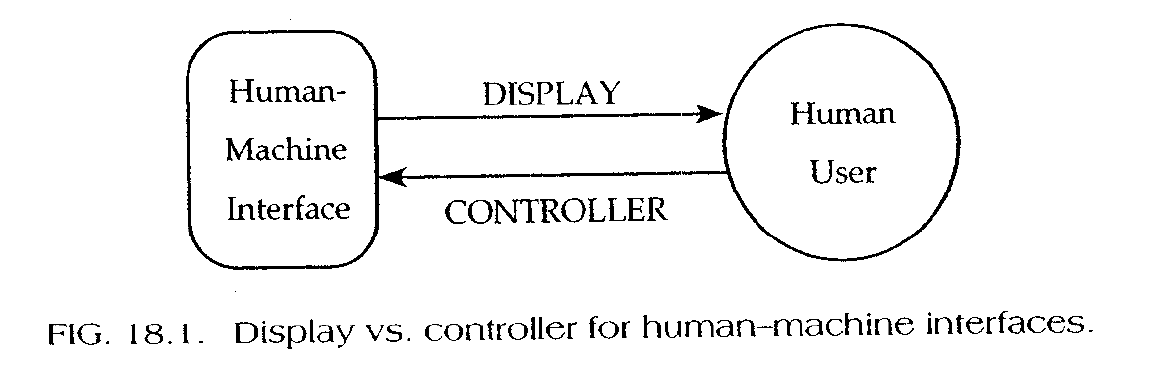
\includegraphics[width = 6cm]{Grafiken/14-Mensch-Maschine.png}
		\caption{Grundlegende Kommunikation zwischen Mensch und Maschine.\cite{Tan:2005:TDS:1198555.1198611}}
		\label{14-Mensch-Maschine}
	\end{center}
\end{figure}

Der Mensch verfügt über einen Tastsinn. Um Informationen über diesen Sinn übertragen zu können, werden haptische Schnittstellen verwendet. 

 %Abschnitt über die Haut
 
Die für den Tastsinn verantwortlichen Nervenzellen können auf unterschiedliche Arten stimuliert werden. Dementsprechen gibt es unterschiedliche haptische Aktuator, die zu Informationsübertragung verwendet werden können. Dabei ist ein Aktuator ein Bauelement, welches elektrische Signale in andere physikalische Größen, wie beispielsweise Bewegung, umsetzt. Dabei ist eine Unterscheidung zwischen Aktuator zu treffen. Die Kommunikation kann entweder über mechanische Bewegung oder elektrische Impulse erfolgen. Darüber hinaus lassen sich weitere Charakteristiken erkennen:

Für beiden Aktuator-Typen vergleichbar sind folgende Charakteristiken:
\begin{itemize}
	\item Position
	
	Die Position gibt den Ort der Stimulation durch den Aktuator an.Die Haut reagiert nicht an jeder Stelle gleich empfindlich auf haptische Stimulation\cite[S.~91]{doi:10.1518/001872008X250638}.
	Die empfindlichsten Stellen liegen in den Fingerspitzen.
	
	\item Berührungsfläche
	Die Berührungsfläche gibt die vom Aktuator Stimulierte Fläche an.
	
	\item Dauer
	
	Die Dauer gibt die zeitliche Länge der Aktivierung des Aktuators an.
\end{itemize}

\begin{figure}[htbp]
	\begin{center}
		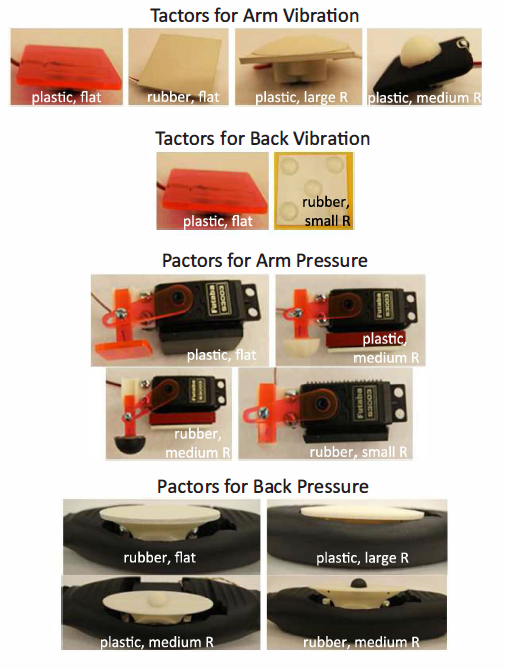
\includegraphics[width = 10cm]{Grafiken/3-Haptische-Aktuatoren.png}
		\caption{Beispiele für haptische Aktuatoren\cite{6183832}. Es liegt eine Unterscheidung von dem Verwendungszweck, dem verwendeten Material und der Form des Materials vor.}
		\label{3-Haptische-Aktuatoren}
	\end{center}
\end{figure}

Für die Kommunikation über Vibrationen\cite{doi:10.1518/001872008X250638}:
\begin{itemize}
	\item Frequenz
	
	Die Frequenz gibt die Anzahl der Wiederholungen des Bewegungszyklus des Aktuators, über einen Zeitraum, an.
	
	\item Amplitude/Intensität %Hier sollte ich mich wahrscheinlich auf eines festlegen
	
	Die Amplitude gibt das Ausrichtungsdelta des Aktuators an.
%Hier könnte vielleicht ein extra Punkt draus gemacht werden. Alternativ kann ich es als Fazit der Kombination der einzelnen Punkte anführen.
\end{itemize}

Für die Kommunikation über elektrische Impulse\cite[S.~4]{68204}:
\begin{itemize}
	\item Stromstärke
	
	Die Stromstärke mit der der elektrische Impuls versetzt wird.
	
	\item Spannung
	
	Die Spannung mit der der elektrische Impuls versetzt wird.
	\item Material
	
	Das Material gibt an, aus welchem Chemischen Stoff die Kontatkfläche des Aktuators aufgebaut ist.
	\item Feuchtigkeit
	
	Die Feuchtigkeit gibt die Menge an vorhandenem Wasser an der Kontaktfläche an. Dabei ist die Leitfähigkeit des Wassers der Grund für diese Charakteristik.
\end{itemize}

In beiden Fällen ist auch die Kombination der einzelnen Faktoren ausschlaggebend, wie effektiv die Kommunikation stattfindet. Dabei stellt jede Ausprägung dieser Kombinationen ein Aktivierungsmuster da. Diese Aktivierungsmuster werden von Menschen nicht nur mit unterschiedlichen Informationen, sondern auch mit subjektiven Emotionen belegt\cite{5444662}.
%Vielleicht nicht hier darstellen, sondern unter eine spezielle Anwendung stellen.

Ein Zusammenschluss von mehreren haptischen Aktuator führt zu einer größeren Anzahl von Einstellungsmöglichkeiten. Diese ermöglichen das übertragen von komplexeren Informationen im Vergleich zu einem haptischen Aktuator. Eine Alternative Einsatzmöglichkeit ist zu der Erhöhung der Redundanz bei der Informationsübertragung. Dabei senden die haptischen Aktuator, beispielsweise, alle das selbe Übertragungsmuster. Das zu erreichene Ziel ist hierbei dem Menschen, der haptische Aktuator auf der Haut trägt, die Aufnahme der Information zu erleichtern. Diese Anwendung ist gerade in kritischen Situationen,wie sie etwa in militärischen Einsätzen zu finden sind, hilfreich\cite{nikolic1998multisensory}. Nikolic et al. \cite{nikolic1998multisensory} beschreibt, wie haptische Aktoren Piloten bei der Überwachung von Flugzeugdaten unterstützen kann.
Je nach Einsatzbereich können zusätzliche Einschränkungen gelten. In dem Bereits angesprochenen Militärbeispiel ist eine Verwendung von Aktoren, die an dem Finger angebracht sind, nicht sinnvoll. Ein Positionierung an den Fingern würde die Verwendung desselben einschränken.

\newpage
\section{Anwendungen}
Nun stellt sich die Frage in welchen Ausprägungen diese Teilgebiete zusammengeführt werden können. Deshalb sollen im folgenden Anwendungen, die alle drei Teilgebiete umfassen beleuchtet werden.

\subsection{Sinneswiederherstellung}
Menschliche Sinne können, von Geburt an oder im laufe der Zeit, nicht, oder nur eingeschränkt, funktionsfähig sein. Um diesen Leistungsverlust ausgleichen zu können bedarf es technischer Hilfsmittel. Hierbei bietet die menschliche Haut eine Möglichkeit zur Aufnahme von Informationen, die typischerweise über andere Sinne aufgenommen werden würden.

\subsubsection{Sehvermögen}
Nach dem Stand der Forschung ist das Auge das Leistungsstärkste Sinnesorgan, gemessen an der übertragenen Datenmenge\cite{Koch2006}. Dabei liegt die absolute Leistung ca. bei der eines Ethernet-Kabels mit 10 Mbit/s\cite{Koch2006}. Der Sehsinn kann somit bereits aus technischen gründen nicht vollständig über die Haut simuliert werden.
Die für die Überwachung der Umwelt wichtigen Informationen lassen sich von den unwichtigen differenzieren.

\subsubsection{Lesen} Geschriebene Worte sind eine Darstellung der menschlichen Sprache. Im Fall der Einschränkung des Sehvermögens ist auch die Fähigkeit zu lesen beeinträchtigt.

\begin{figure}[htbp]
	\begin{center}
		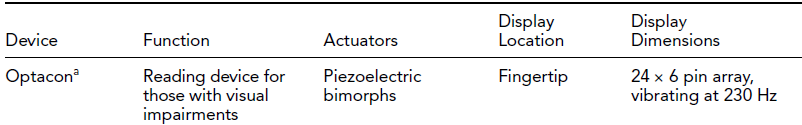
\includegraphics[width = 12cm]{Grafiken/4-Optacon-Data.png}
		\caption{Rahmendaten des Optacons.\cite{doi:10.1518/001872008X250638}}
		\label{4-Optacon-Data}
	\end{center}
\end{figure}

\paragraph{Optacon} Eine Lösung für diese Einschränkung wurde von Bliss et al. 1970 in Form des ''Optacon'' entwickelt (Zitiert nach:\cite{doi:10.1518/001872008X250638}). Dabei werden auf einer Anzeigefläche die Buchstaben in Form von Vibrationen dargestellt. Das identifiezieren der Buchstaben übernimmt ein Scanner, der über geschrieben Worte bewegt werden kann. Mit diesem Gerät ist war es möglich zwischen 50 und 100 Worte in der Minute zu lesen \cite{doi:10.1518/001872008X250638}.
Bliss et al. \cite{4081931} identifiert in seiner Arbeit drei Tests Charakteristiken, die einen Einblick in die Leistung eines "Direkt Übersetzers mit taktilem Ausgang" \cite{4081931} bieten.

\begin{itemize}
	\item Lesbarkeit\newline Die Lesbarkeit beschreibt, mit welcher Wahrscheinlichkeit, die gelesene Information von dem Benutzer, wie vorgesehen interpretiert wird. Für das Erreichen der Charakteristik muss es möglich sein Buchstaben zu unterscheiden. Auch ist die Erneuerungsrate, mit dem das Gerät die Buchstaben neu zeichnet, von Bedeutung. Eine zu geringe Wiederholungsrate kann zu Missverständnissen führen.
	
	\item Lesegeschwindigkeit\newline
	Die Lesegeschwindigkeit gibt an, wie schnell Wörter bzw. Buchstaben gelesen werden können. Diese Charakteristik hängt mit dem Trainingsstand des Anwenders zusammen.
	
	\item Lesbarer Ausschnitt\newline
	In dem Lesbaren Ausschnitt können Buchstaben willkürlich erkannt werden. Je größer dieser Ausschnitt ist, desto länger kann ein Anwender lesen ohne Änderungen an einem Gerät vorzunehmen.
\end{itemize}


\subsection{Zwischenmenschliche Kommunikation}

Die Zwischenmenschliche Kommunikation ist ein komplexer Vorgang, bei dem zumeist viele Sinne beansprucht werden. Über den Hörsinn werden die Informationen aufgenommen, die in der gesprochenen Sprache zu finden sind. Der Sehsinn wird verwendet um Lippen zu lesen und somit ein besseres Verständnis zu erzeugen. Darüber hinaus kann über ihn die emotionale Lage des Gesprächspartners eingeschätzt werden und auf Gesten, wie ein Handschlag, reagiert werden.
Jedoch gibt es auch Umgebungen, in denen diese Kommunikationswege unterbunden werden. Der Geräuschpegel kann zu hoch sein um Sprache zu verstehen. Die Lichtverhältnisse können zu dunkel sein um den anderen Menschen zu sehen, mit dem Kommuniziert wird \cite{10.2307/1705360}.

Des weiteren können auch durch Unfälle, Alter oder Krankheiten die Augen und Ohren beeinträchtigt sein. Um die Fähigkeit der Zwischenmenschlichen Kommunikation zu erhalten sind Seh- und Hörhilfen verbreitete technische Werkzeuge. Eine weitere Alternative ist das Umverlagern der Kommunikation auf einen anderen Sinn\cite{10.2307/1705360}.

Frank A. Geldard \cite{10.2307/1705360} beschreibt hierzu in seiner Arbeit die Entwicklung der Forschung, die versucht die zwischenmenschliche Kommunikation auf den Tastsinn zu verlagern. Zuerst wird beschrieben, wie die Haut dazu genutzt werden kann wie ein Ohr zu funktionieren. Dabei wird die Haut als Trommelfell verwendet. Dieser Ansatz liefert nach einer Einlernphase von 30h ein Vokabular von einigen einzelnen Worten\cite{10.2307/1705360}. Das Problem bei dieser Anwendung liegt in der Zuverlässigkeit. Bei einer Wiederkennungsrate von ca. 75% ist die Wahrscheinlichkeit, dass die gesagten Worte nicht oder falsch verstanden werden hoch\cite{10.2307/1705360}. Eine Lösung für dieses Problem kann das Abändern des Vokabulares sein. Anstelle, dass Buchstaben übertragen werden können auch Vibrationsbilder übermittelt werden\cite{10.2307/1705360}.

\paragraph{Tactons} Die Idee, für die haptische Wahrnehmung spezialisierte Vibrationsmuster zu erstellen, wird von Stephen Brewster und Lorna M. Brown\cite{Brewster:2004:TST:976310.976313} behandelt. Ihr Vorschlag ist sogenannte Tactile Icons (Tactons) zu verwenden, die haptisch gut differenzierbar sind. Dabei orientieren sie sich an musik ähnlichen Mustern, die von den taktilen Aktoren dargestellt werden\cite{Brewster:2004:TST:976310.976313}.
Der Unterschied zu der Darstellung von Buchstaben ist, dass die Tactons selbst eine Bedeutung haben und nicht in eine gesprochene Sprache übersetzt werden müssen um sie zu verstehen. Dadurch sollte eine bessere Antwortzeit bei dem Benutzer erreicht werden. Wie in \ref{7-Tacton-Verwendungsbeispiel} sichtbar.

\begin{figure}[htbp]
	\begin{center}
		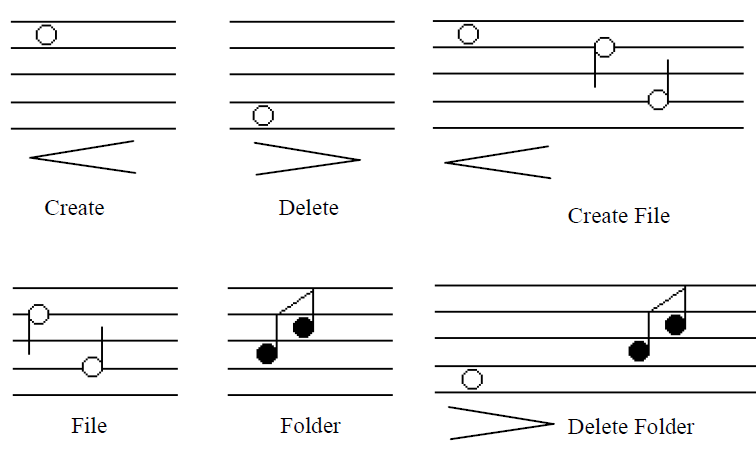
\includegraphics[width = 8cm]{Grafiken/7-Tacton-Verwendungsbeispiel.png}
		\caption{Codierung von Informationen über einen Tacton\cite{Brewster:2004:TST:976310.976313}. Dabei wird eine Notation ähnlich zur Musik verwenet um Frequenz und Amplitude anzugeben.}
		\label{7-Tacton-Verwendungsbeispiel}
	\end{center}
\end{figure}

\subsection{Leistungssteigerung}

\begin{figure}[htbp]
	\begin{center}
		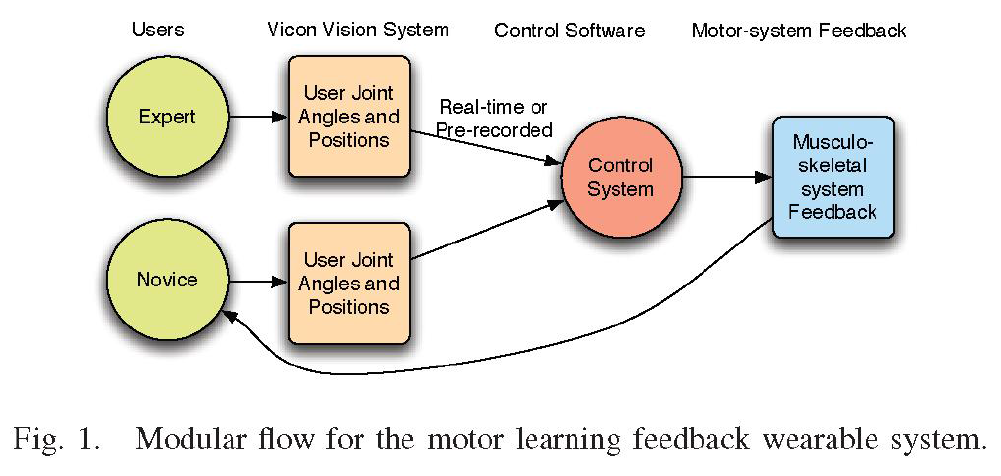
\includegraphics[width = 10cm]{Grafiken/17-Lehrnbeschleunigung-Versuchsaufbau.png}
		\caption{Aufbau des Experiments zur Lehrnbeschleunigung durch haptische Schnittstellen\cite{lieberman2007development}.}
		\label{17-Lehrnbeschleunigung-Versuchsaufbau}
	\end{center}
\end{figure}

Auf der Basis von\cite{rupert2000instrumentation},\cite{calhoun2002utilty}
Am wichtigsten ist \cite{lieberman2007development}

\subsection{Erweiterung des Wahrnehmungsspektrums}

\paragraph{Navigationssysteme}

\begin{figure}[htbp]
	\begin{center}
		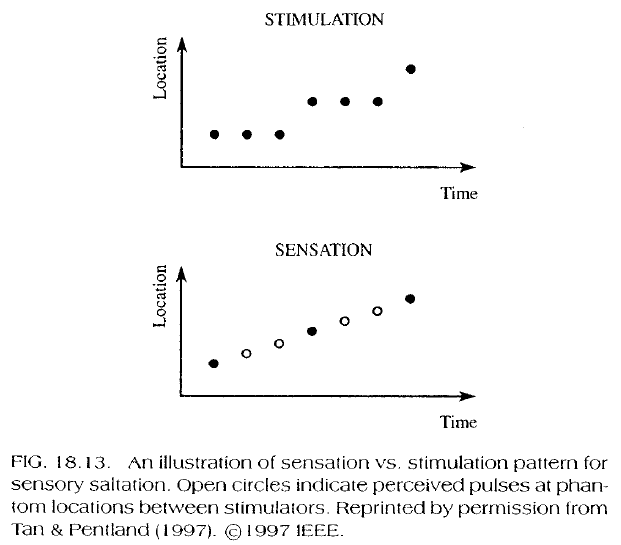
\includegraphics[width = 10cm]{Grafiken/14-Sensory-Saltation.png}
		\caption{ToDo}
		\label{14-Sensory-Saltation}
	\end{center}
\end{figure}
\subsection{Zuverlässigkeit Erzeugung}
Haptische Aktuatoren bieten die Möglichkeit Informationen redundant dazustellen. So können Informationen, die von einem Display abgelesen werden, zusätzlich haptisch unterstützt werden. Dies ist ein Vorgehen, dass bei Piloten zu dem Einsatz kommt.
Anius H. Rupert\cite{rupert2000instrumentation} beschreibt in seiner Arbeit das Problem der räumliche Desorientierung bei Piloten, die keinen Horizont als Referenz zur Verfügung haben. Dies führt zu einem Verlust der Orientierung und somit zu einem Kontrollverlust über das Flugzeug. Eine Lösung Stellt das "Tactical Situation Awareness System (TSAS)"\cite{rupert2000instrumentation} da. Dabei wird der visuelle Horizont durch haptisches Feedback simuliert\cite{rupert2000instrumentation}. Im Falle einer visuellen Einschränkung ist der Pilot somit nicht mehr ausschließlich auf seine Augen beschränkt.
Aus diesem Beispiel der Anwendung von Redundanz zu der Erhöhung der Zuverlässigkeit in Beobachtungsaufgaben lassen sich einige allgemeine Schlüsse ziehen:

\begin{figure}[htbp]
	\begin{center}
		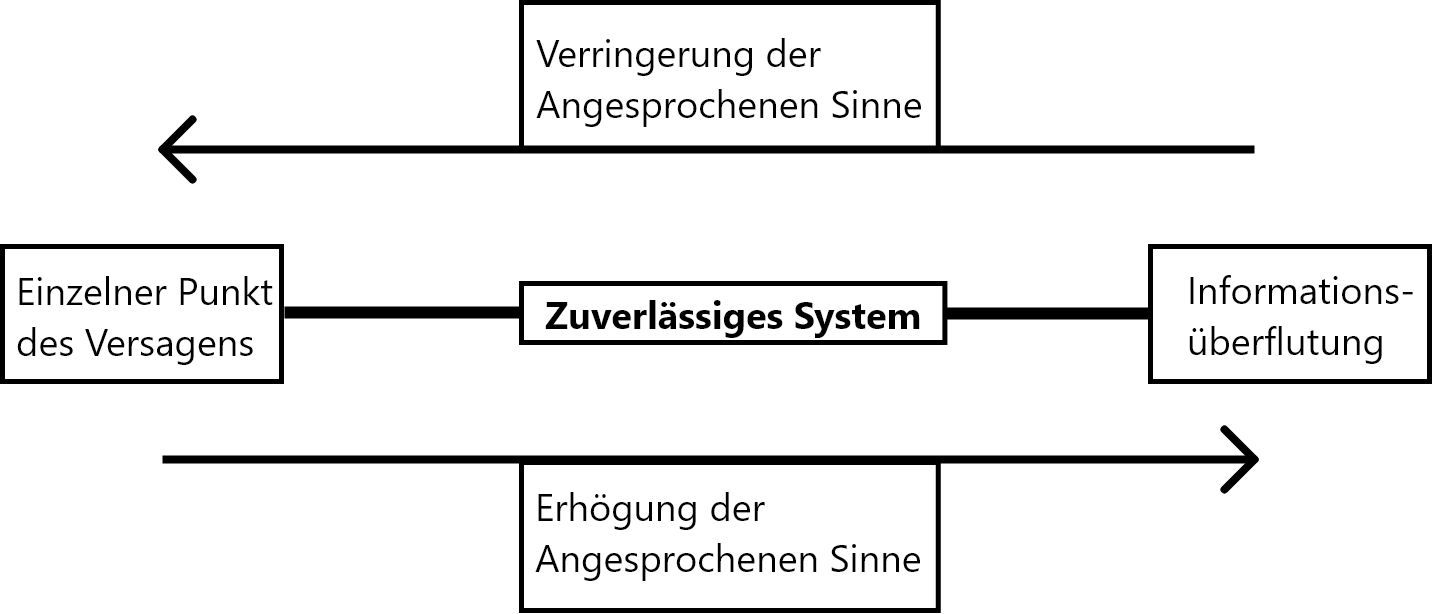
\includegraphics[width = 10cm]{Grafiken/Sinne-Redundanz-Verhaeltnis.png}
		\caption{Ein naiver Ansatz für die Beschreibung der Zusammenhänge von der Anzahl der angesprochenen Sinnen im Verhältnis zu der Zuverlässigkeit.}
		\label{Sinne_Redundanz_Verhaeltnis}
	\end{center}
\end{figure}


%Fokusschreiben
Es lässt sich für jedes Monitoring Problem festhalten, dass eine Konkurrenz um die Aufmerksamkeit stattfindet. Dabei ist es jedoch nicht so, dass die Aufmerksamkeit eine limitierte Ressource ist. Vielmehr tritt sie bei der richtigen Stimulation hervor. So kann bsp. eine visuelle Darstellung alleine nicht interessant genug sein, um die Aufmerksamkeit zu fesseln, aber in Kombination mit einer auditoren oder haptischen Stimulation schon. Auf der Anderen Seite des Spektrums bewegt sich die Überreizung. In ihr gehen Nouancen durch zu viele Informationen verloren.
Es muss also zuerst festgestellt werden, ob das Problem ein Mangel an Information, die interessant sind, ist, oder ob eine Reizüüberflutung stattfindet. Bei dem Pilotenbeisbiel ist es eine Reizüüberflutung. Der Pilot muss viele Informationen buchstäblich im Blick behalten. Dadurch kann die Anzeige überfüllt und schwer zu differenzieren sein. Eine weitere haptische Stimulation ermöglicht es daher die Information entweder zu unterstreichen, oder erst dazustellen. Das Isolierte Darstellen spart Platz auf dem Display. Jedoch stellt es einen Singel Point of Failure da. Wenn also die Information entweder übersehen wird, oder ein Äußerer Zustand als diese Information eingeschätzt wird, so kann es schnell zu Problemen führen. Eine Erhöhung der Redundanz kann, wenn es übertrieben wird ablenkend sein. Zum Beispiel, wenn ein Pilot durch die Vibration so stark erschrocken wird, dass er für mehrere Sekunden andere, potentiell wichtigere Informationen übersieht. Deshalb halte ich eine Limitierung auf zwei Faktoren für die Selbe Information im Pilotenbeispiel für sinnvoll. Acuh ist zu berücksichtigen, dass die Einflussfaktoren, die man zur Verfügung hat nicht für alle Aufgaben gleich gut geeignet sind. Die Amplitude zu Ändern beispielsweise isit schwer zu erkenn. Leichter ist es die Dauer bzw. Lokation zu differenzieren.
\newpage
\section{Zusammenfassung und Ausblick}

%Zusätzliche Informationen und Formalitäten
\newpage
\section{Anhang}

\begin{figure}[htbp]
	\begin{center}
		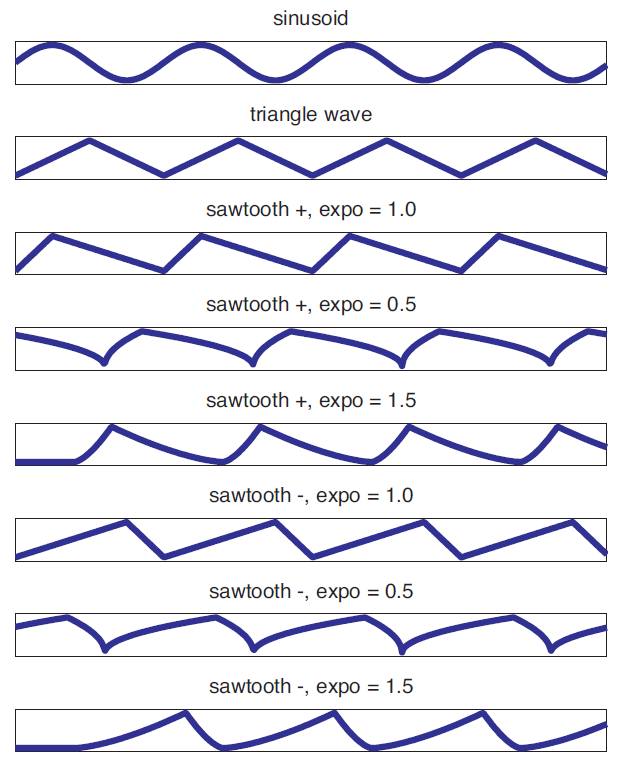
\includegraphics[width = 5cm]{Grafiken/2-Aktivierungsprofile.png}
		\caption{Beispiel für Bewegungsmuster eines Vibrations Aktuators\cite{5444662}. }
		\label{2-Aktivierungsprofile.png}
	\end{center}
\end{figure}

\begin{figure}[htbp]
	\begin{center}
		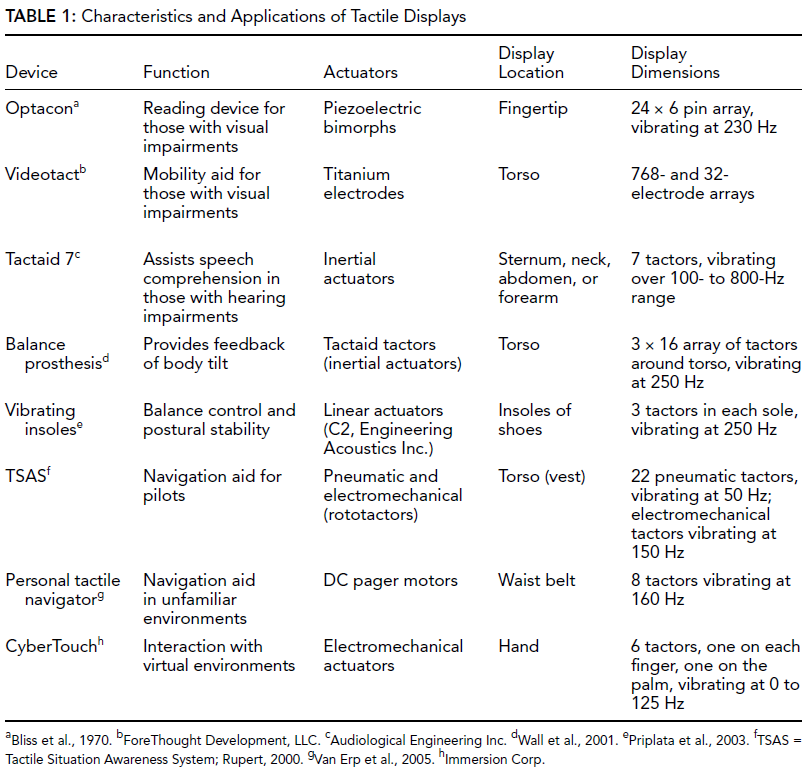
\includegraphics[width = 10cm]{Grafiken/4-Uebersicht-Projekte.png}
		\caption{ToDo}
		\label{4-Uebersicht-Projekte}
	\end{center}
\end{figure}

\begin{figure}[htbp]
	\begin{center}
		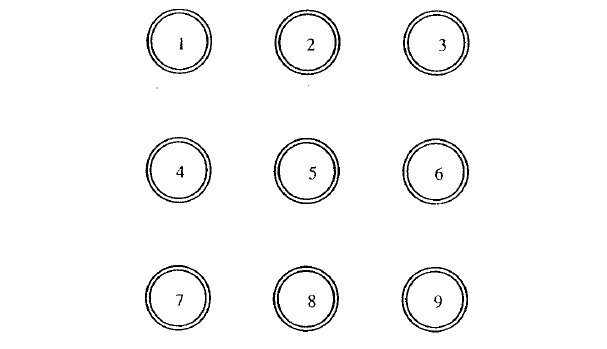
\includegraphics[width = 10cm]{Grafiken/14-3x3-Grid.png}
		\caption{ToDo}
		\label{14-3x3-Grid}
	\end{center}
\end{figure}

\begin{figure}[htbp]
	\begin{center}
		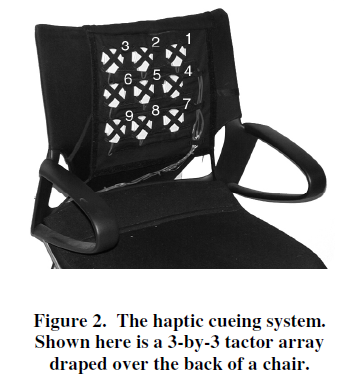
\includegraphics[width = 10cm]{Grafiken/21-Haptic-System-3x3.png}
		\caption{ToDo}
		\label{21-Haptic-System-3x3}
	\end{center}
\end{figure}

\begin{figure}[htbp]
	\begin{center}
		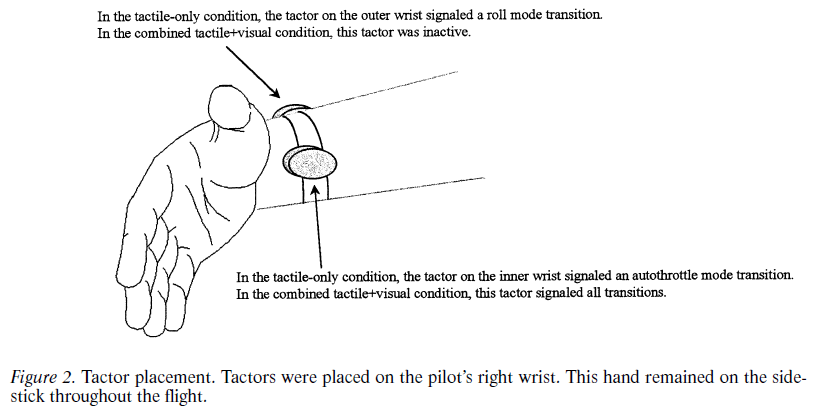
\includegraphics[width = 10cm]{Grafiken/25-Tactor-Placement-Good-Vibration.png}
		\caption{ToDo}
		\label{25-Tactor-Placement-Good-Vibration}
	\end{center}
\end{figure}

\begin{figure}[htbp]
	\begin{center}
		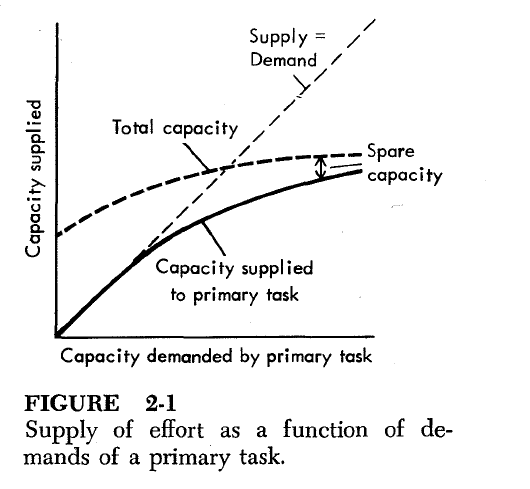
\includegraphics[width = 10cm]{Grafiken/28-Attetntion-Reserves.png}
		\caption{ToDo}
		\label{28-Attetntion-Reserves}
	\end{center}
\end{figure}

%Template für Bilder
%\begin{figure}[htbp]
%	\begin{center}
%		\includegraphics[width = 10cm]{Grafiken/ToDo.png}
%		\caption{ToDo}
%		\label{ToDo}
%	\end{center}
%\end{figure}

\subsection{Selbständigkeitserklärung}

\clearpage
\bibliography{Literaturreferenzen}

\end{document}
